\chapter{Supplementary information}

\begin{figure}[htbp]
    \centering
    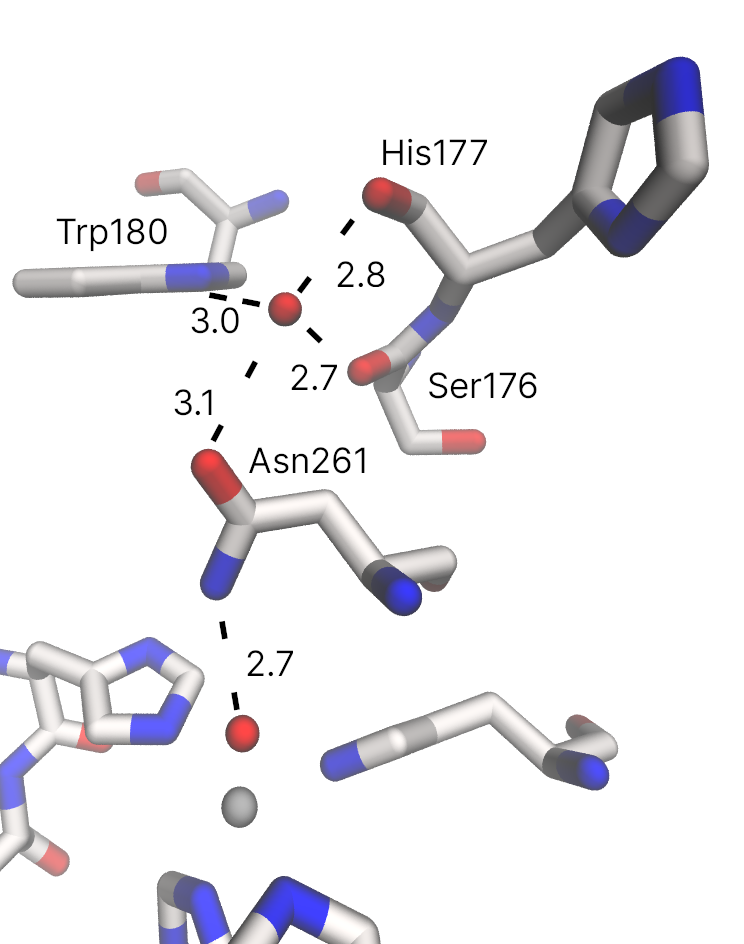
\includegraphics[width=0.5\textwidth]{Figures/crystal_water.png}
    \caption{Hydrogen bond network around the conserved Asn261 residue in the crystal structure of mouse SCD1 (PDB: 4YMK, \cite{Bai2015}). Based on the network, the other Asn rotamer should be more favorable. Colours: silver, zinc; red, oxygen; blue, nitrogen; white, carbon.}
    \label{fig:Crystal_water}
\end{figure}

\begin{table}[htbp]
\centering
\caption{Reactivity of rat stearoyl-CoA desaturase with different acyl-CoA substrates. $K_{m}$ and the Relative maximal velocity are determined by Lineweaver-Burk plots. Some $K_{m}$ values are not measured due to low activity. Adapted from \cite{Enoch1976}.}
\scalebox{0.8}{\begin{tabular}{@{}lcc@{}}
\toprule
\multicolumn{1}{c}{Compound tested} & $K_m$      & \begin{tabular}[c]{@{}c@{}}Relative\\ maximal\\ velocity\end{tabular} \\ \midrule
                                    & $\mu M$    & \%                                                                    \\
Decanoyl-CoA                        & -          & \textless 1                                                           \\
Dodecanoyl-CoA                      & -          & 7                                                                     \\
Tridecanoyl-CoA                     & 8.0        & 50                                                                    \\
Tetradecanoyl-CoA                   & 4.7        & 69                                                                    \\
Hexadecanoyl-CoA (palmitoyl-CoA)    & 4.7        & 86                                                                    \\
Heptadecanoyl-CoA                   & 5.0        & 103                                                                   \\
Octadecanoyl-CoA (stearoyl-CoA)     & 4.5        & 100                                                                   \\
Nonadecanoyl-CoA                    & 5.0        & 103                                                                   \\
Eicosanoyl-CoA (20:0)               & -          & \textless 1                                                           \\ \bottomrule
\end{tabular}}
\label{tab:Enoch_table}
\end{table}

\begin{figure}[htbp]
    \centering
    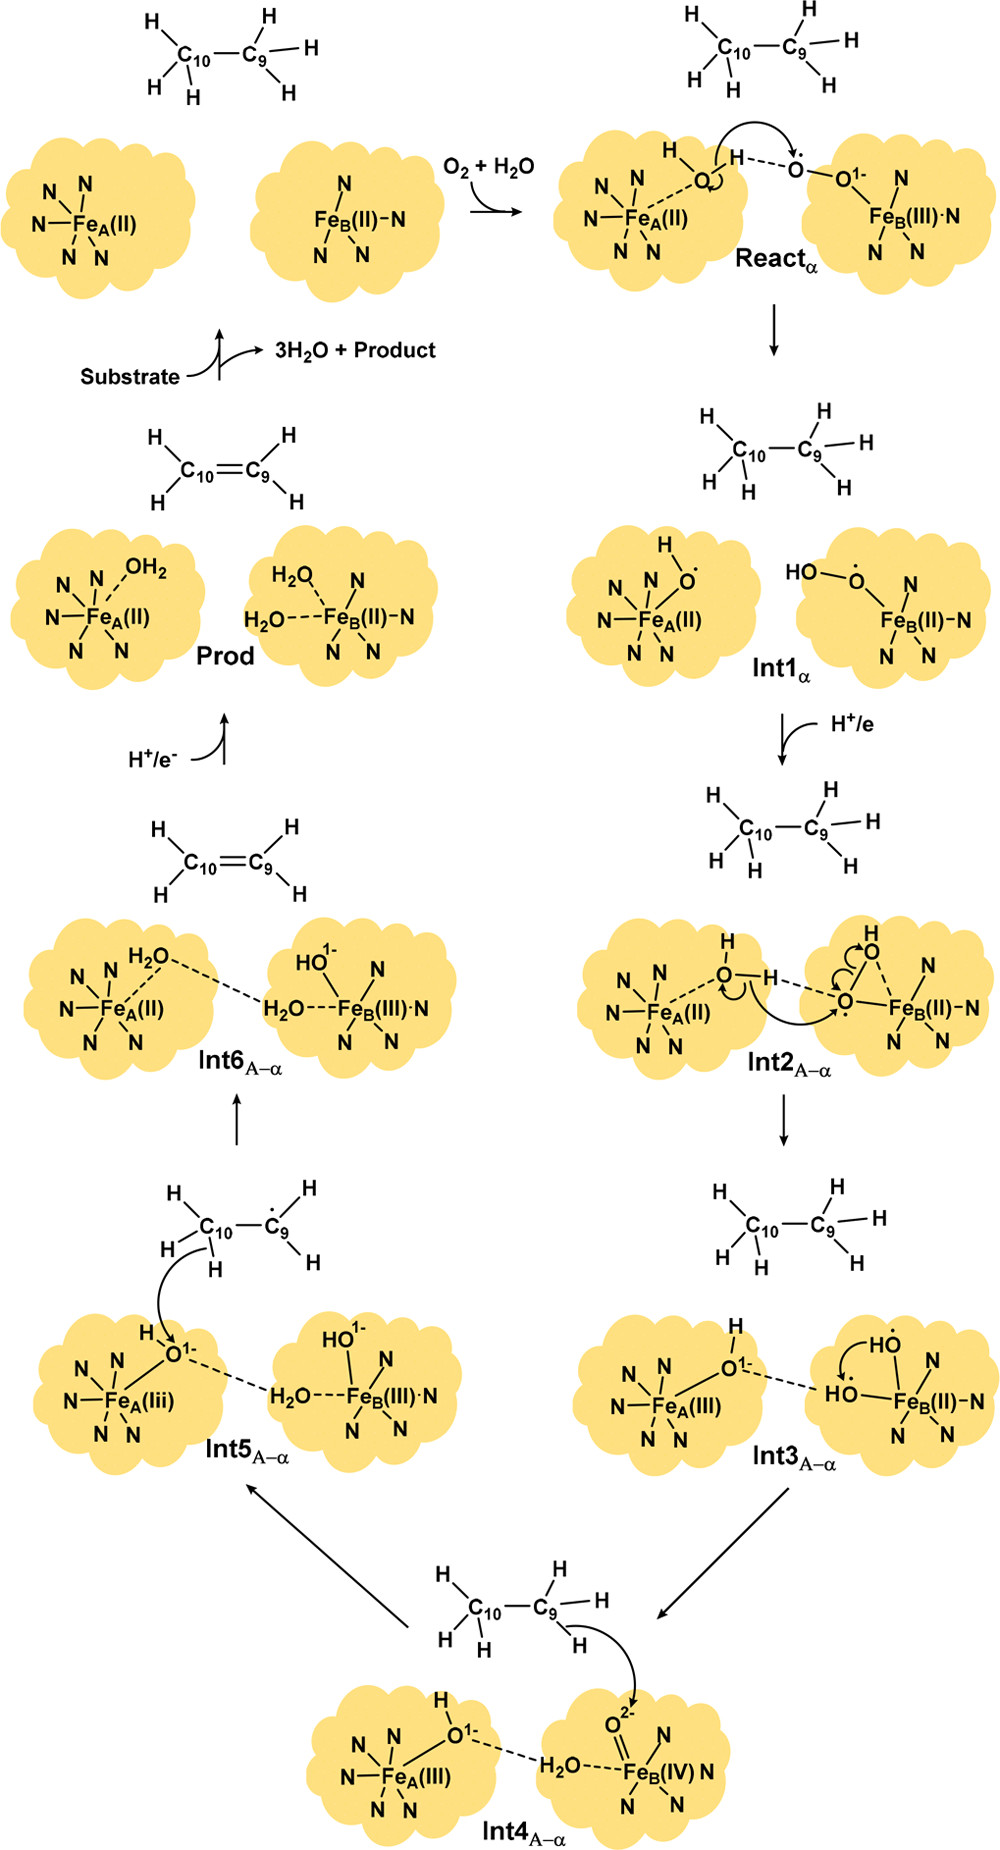
\includegraphics[width=0.65\textwidth]{Figures/Yu_mechanism.jpeg}
    \caption{Proposed reaction mechanism of stearoyl-CoA desaturase based on a cluster model DFT/B3LYP study. Directly taken from \cite{Yu2019}. Note: the exact characterisation of the shown species is not always completely clear. For example, Int3$_{A-\alpha}$ on Fe$_{\text{B}}$ is shown as a dihydroxyl Fe$_{\text{B}}$(II)$-$($\cdot$OH)$_2$ radical but it also has dihydroxo Fe$_{\text{B}}$(IV)$-$(OH)$_{2}^{2-}$ character, so the process from Int3$_{A-\alpha}$ to Int4$_{A-\alpha}$ can be described either as an internal proton transfer or hydrogen atom transfer. In this thesis Int4$_{A-\alpha}$ is referred to as intermediate A.}
    \label{fig:SCD1_mechanism}
\end{figure}


\begin{table}[htbp]
\caption{Equilibration protocol used for classical molecular dynamics simulations of SCD1.}
\centering
\scalebox{0.8}{\begin{tabular}{@{}ccccccc@{}}
\toprule
Run & Calculation type        & Restraints {[}kcal/mol $^2${]}                                                           & Constant & \begin{tabular}[c]{@{}c@{}}Minimization steps / \\ simulation time\end{tabular} & Shake & Timestep {[}fs{]} \\ \midrule
1   & minimization (CPU)      & \begin{tabular}[c]{@{}c@{}}whole protein (100)\\ ST9 (100)\\ membrane (100)\end{tabular} & V        & 1000 steps                                                                      & No    & -                 \\ \midrule
2   & minimization (GPU)      & \begin{tabular}[c]{@{}c@{}}whole protein (100)\\ ST9 (100)\\ membrane (100)\end{tabular} & V        & 10 000 steps                                                                    & No    & -                 \\ \midrule
3   & minimization (CPU)      & \begin{tabular}[c]{@{}c@{}}whole protein (100)\\ ST9 (100)\end{tabular}                  & V        & 1000 steps                                                                      & No    & -                 \\ \midrule
4   & minimization (GPU)      & \begin{tabular}[c]{@{}c@{}}whole protein (100)\\ ST9 (100)\end{tabular}                  & V        & 10 000 steps                                                                    & No    & -                 \\ \midrule
5   & minimization (CPU)      & -                                                                                        & V        & 10 000 steps                                                                    & No    & -                 \\ \midrule
6   & heating (CPU) 0-100 K   & \begin{tabular}[c]{@{}c@{}}whole protein (5)\\ ST9 (5)\\ membrane (5)\end{tabular}       & V        & 5 ps                                                                            & Yes   & 1                 \\ \midrule
7   & heating (GPU) 100-300 K & \begin{tabular}[c]{@{}c@{}}whole protein (5)\\ ST9 (5)\\ membrane (5)\end{tabular}       & P        & 100 ps                                                                          & Yes   & 1                 \\ \midrule
8   & equilibration (GPU)     & \begin{tabular}[c]{@{}c@{}}whole protein (5)\\ ST9 (5)\end{tabular}                      & P        & 1 ns                                                                            & Yes   & 1                 \\ \midrule
9   & equilibration (GPU)     & \begin{tabular}[c]{@{}c@{}}backbone (5)\\ ST9 (5)\end{tabular}                           & P        & 1 ns                                                                            & Yes   & 1                 \\ \midrule
10  & equilibration (GPU)     & \begin{tabular}[c]{@{}c@{}}alpha carbons (5)\\ ST9 (5)\end{tabular}                      & P        & 1 ns                                                                            & Yes   & 1                 \\ \midrule
11  & equilibration (GPU)     & -                                                                                        & P        & 1 ns                                                                            & Yes   & 1                 \\ \midrule
12  & equilibration (GPU)     & -                                                                                        & P        & 5 ns                                                                            & Yes   & 2                 \\ \bottomrule
\end{tabular}}
\label{tab:eq_protocol}
\end{table}

\begin{figure}[htbp]
    \centering
    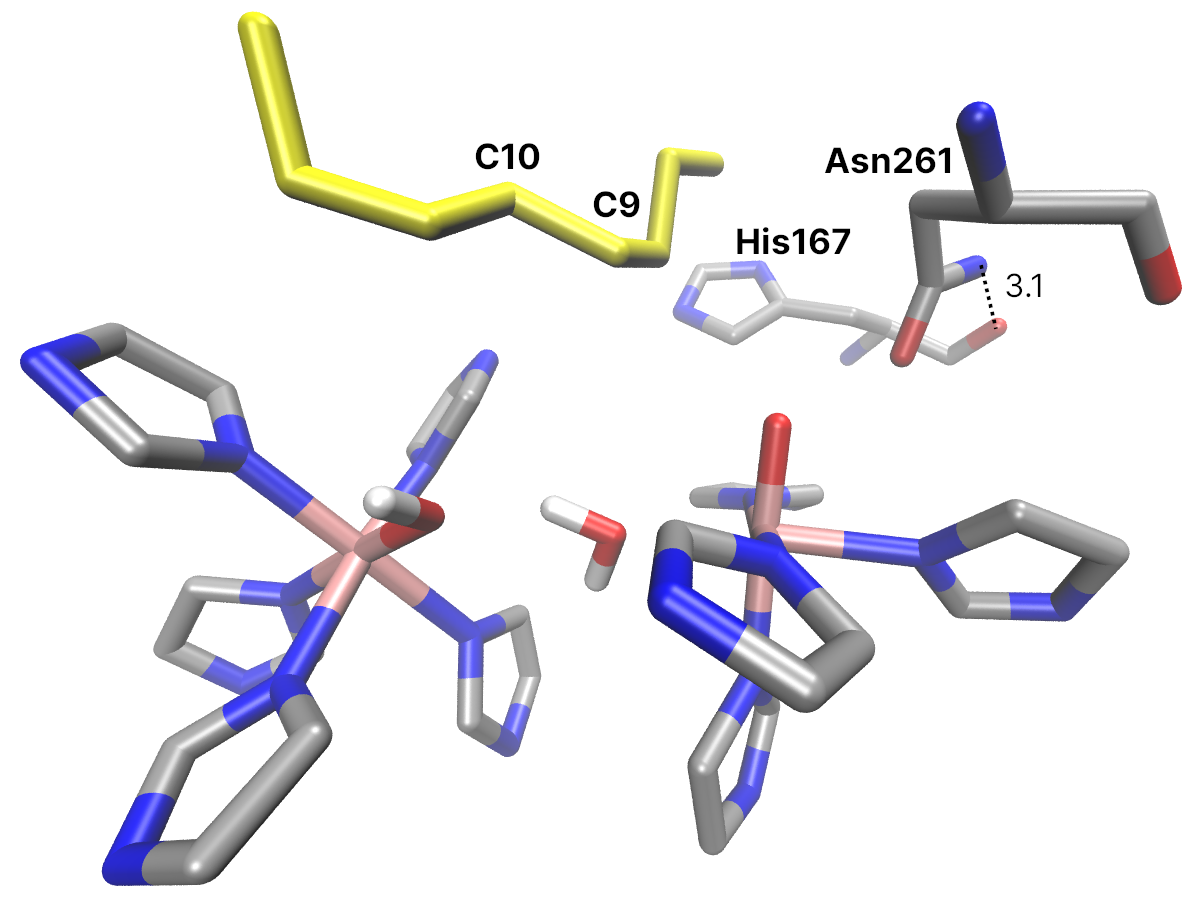
\includegraphics[width=0.8\textwidth]{Figures/int_A_run2.png}
    \caption{Structure of the active site during the second MD production run of intermediate A. Residues are shown as sticks. Distances are shown in Å. Colours: silver, protein carbons; red, oxygen; blue, nitrogen; white, hydrogen; yellow, carbons of stearoyl-CoA; pink, iron. Hydrogen atoms are left out for clarity.}
    \label{fig:intA_run2}
\end{figure}

\begin{figure}[htbp]
    \centering
    \begin{subfigure}{.49\textwidth}
        \centering
        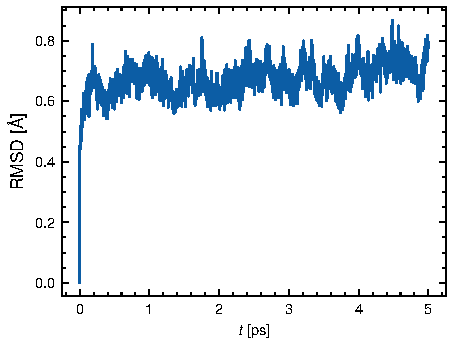
\includegraphics[width=\textwidth]{Figures/B_rmsd.pdf}
    \end{subfigure}
    \begin{subfigure}{.49\textwidth}
        \centering
        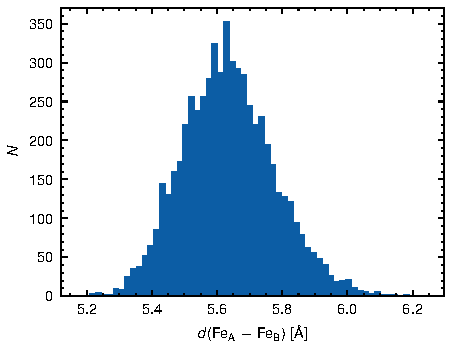
\includegraphics[width=\textwidth]{Figures/B_fe-fe_hist.pdf}
    \end{subfigure}
    \par\bigskip
    \begin{subfigure}{.49\textwidth}
        \centering
        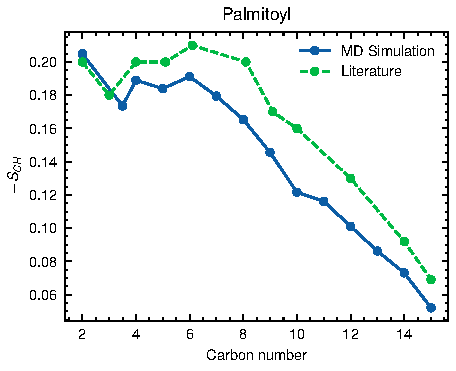
\includegraphics[width=\textwidth]{Figures/B_palmitoyl.pdf}
    \end{subfigure}
    \begin{subfigure}{.49\textwidth}
        \centering
        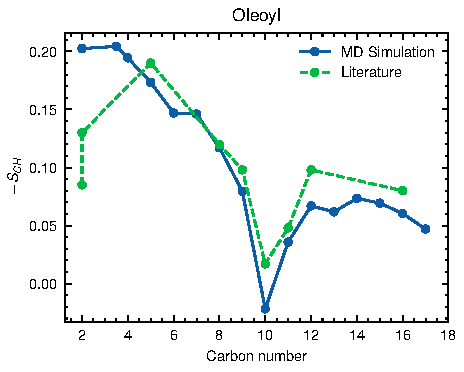
\includegraphics[width=\textwidth]{Figures/B_oleoyl.pdf}
    \end{subfigure}
    \caption{Data to assess the equilibration of intermediate B taken from the last 5 ns equilibration run. RMSD of the protein's backbone alpha carbon atoms with respect to the first frame (top left). Distribution of the iron-iron distance (top right). Average lipid order parameters for the palmitoyl chain of POPC (bottom left). Average lipid order parameters for the oleoyl chain of POPC (bottom right). Experimental values for the lipid order parameters are taken from \cite{Seelig1978,Perly1985}.}
    \label{fig:B_equilibration}
\end{figure}


\begin{figure}[htbp]
    \centering
    \begin{subfigure}{\textwidth}
        \centering
        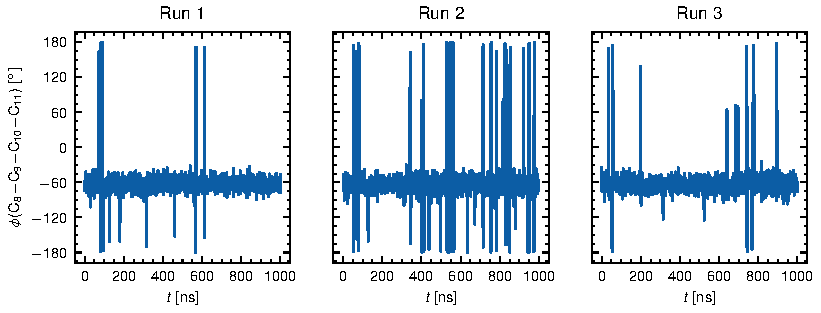
\includegraphics[width=\textwidth]{Figures/B_C9-C10_all.pdf}
    \end{subfigure}
    \par\bigskip
    \begin{subfigure}{\textwidth}
        \centering
        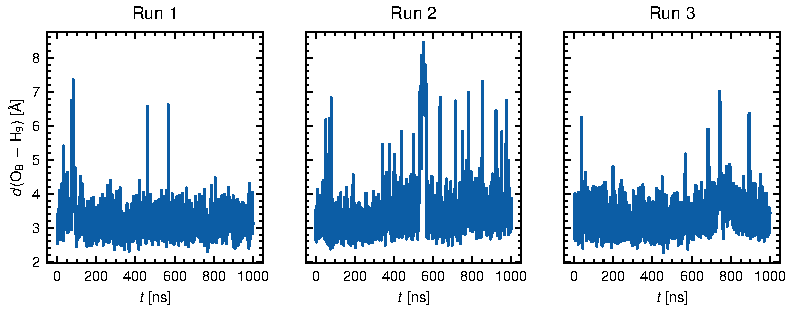
\includegraphics[width=\textwidth]{Figures/B_Ob-H9_all.pdf}
    \end{subfigure}
    \par\bigskip
    \begin{subfigure}{\textwidth}
        \centering
        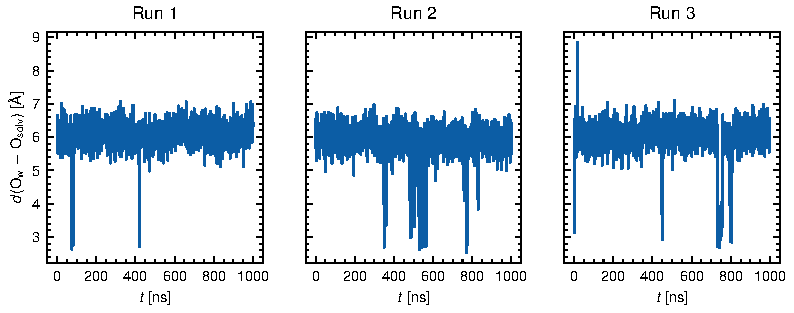
\includegraphics[width=\textwidth]{Figures/B_Ow-Ow_all.pdf}
    \end{subfigure}
    \caption{Data from the three 1 $\mu$s production runs of intermediate B: value of the C$_8-$C$_9-$C$_{10}-$C$_{11}$ dihedral angle of the substrate (top); distance between the oxo oxygen (O$_{\text{B}}$) and \textit{pro}-R hydrogen on C$_9$ (H$_{9}$) that needs to get abstracted (middle); distance between the oxygen of the active site water ligand (O$_{\text{W}}$) and oxygen of a nearby solvent water molecule in the substrate tunnel (bottom). Note: due to the cyclical nature of the dihedral angles the values around 180$^{\circ}$ and $-$180$^{\circ}$ correspond to the same \textit{anti} conformation.}
    \label{fig:B_appendix}
\end{figure}

\begin{figure}
    \centering
    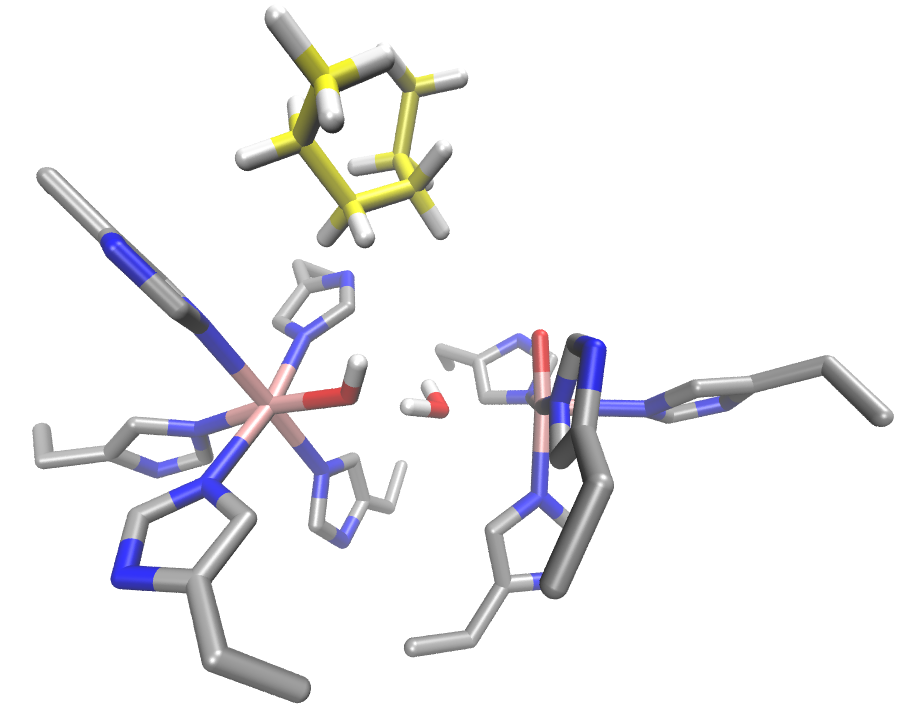
\includegraphics[width=0.7\textwidth]{Figures/intA_xtb.png}
    \caption{Structure of intermediate A after optimization with GFN2-xTB. Residues are shown as sticks. Distances are shown in Å. Colours: silver, protein carbons; red, oxygen; blue, nitrogen; white, hydrogen; yellow, carbons of stearoyl-CoA; pink, iron. Protein's hydrogen atoms are left out for clarity.}
    \label{fig:xtb_intA}
\end{figure}

\begin{figure}
    \centering
    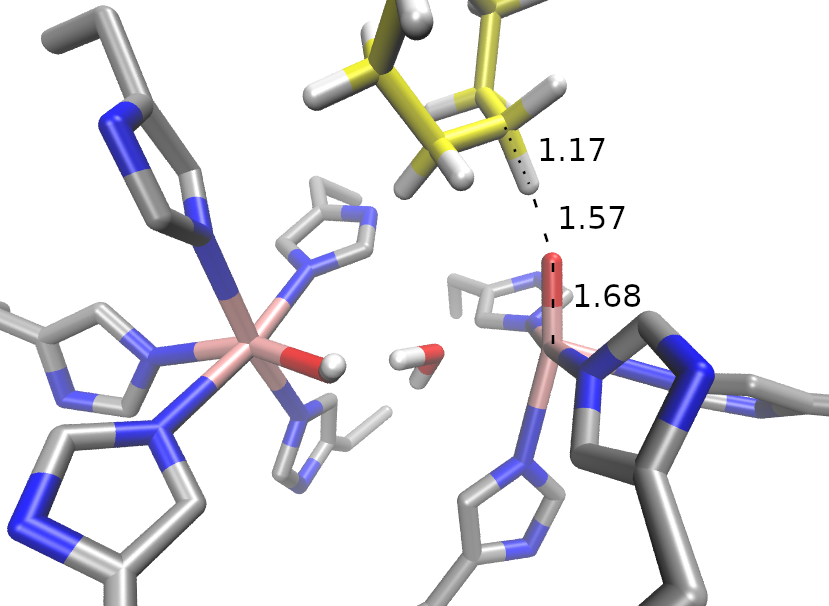
\includegraphics[width=0.7\textwidth]{Figures/TS_xtb.png}
    \caption{Structure of the predicted TS from the GFN2-xTB cluster model PES scan. Residues are shown as sticks. Distances are shown in Å. Colours: silver, protein carbons; red, oxygen; blue, nitrogen; white, hydrogen; yellow, carbons of stearoyl-CoA; pink, iron. Protein's hydrogen atoms are left out for clarity.}
    \label{fig:xtb_TS}
\end{figure}

\begin{table}[htbp]
\caption{Spin densities of the TS predicted by the GFN2-xTB cluster model relaxed potential energy surface scan of intermediate A. Predicted values with B3LYP are taken from \cite{Yu2019}.}
\centering
\begin{tabular}{@{}ccc@{}}
\toprule
\textbf{Atom} & \textbf{\textit{S}$_\text{B3LYP}$} & \textbf{\textit{S}$_\text{GFN2-xTB}$} \\ \midrule
Fe$_{\text{A}}$           & 4.14            & 3.86               \\ \midrule
O$_{\text{A}}$             & 0.27            & 0.25               \\ \midrule
Fe$_{\text{B}}$            & -3.80           & 2.72               \\ \midrule
O$_{\text{B}}$             & -0.25           & 0.64               \\ \midrule
C$_{\text{9}}$             & 0.30            & 0.20               \\ \bottomrule
\end{tabular}
\label{tab:xtb_spin}
\end{table}

\begin{figure}[htbp]
    \centering
    \begin{subfigure}{.49\textwidth}
        \centering
        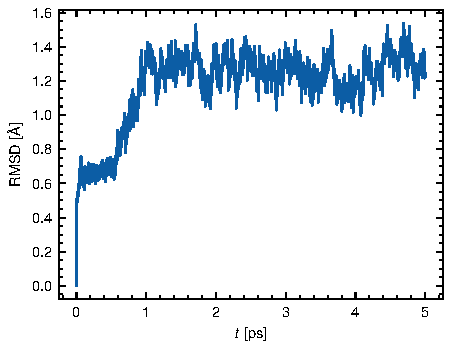
\includegraphics[width=\textwidth]{Figures/TIP3P_rmsd.pdf}
    \end{subfigure}
    \begin{subfigure}{.49\textwidth}
        \centering
        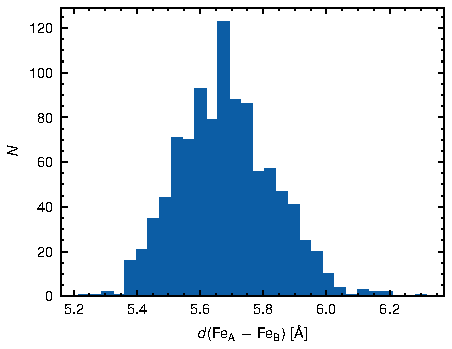
\includegraphics[width=\textwidth]{Figures/TIP3P_fe-fe_hist.pdf}
    \end{subfigure}
    \par\bigskip
    \begin{subfigure}{.49\textwidth}
        \centering
        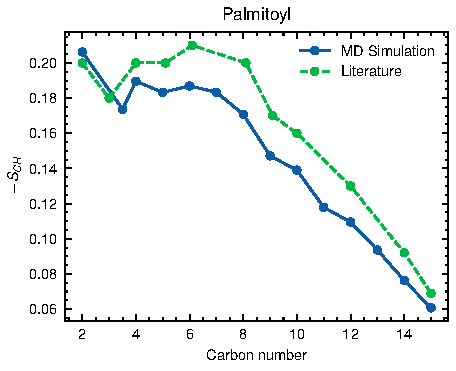
\includegraphics[width=\textwidth]{Figures/TIP3P_palmitoyl.pdf}
    \end{subfigure}
    \begin{subfigure}{.49\textwidth}
        \centering
        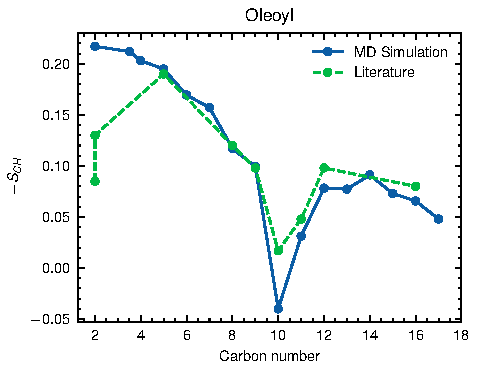
\includegraphics[width=\textwidth]{Figures/TIP3P_oleoyl.pdf}
    \end{subfigure}
    \caption{Data to assess the equilibration of intermediate B with the TIP3P water model taken from the last 5 ns equilibration run. RMSD of the protein's backbone alpha carbon atoms with respect to the first frame (top left). Distribution of the iron-iron distance (top right). Average lipid order parameters for the palmitoyl chain of POPC (bottom left). Average lipid order parameters for the oleoyl chain of POPC (bottom right). Experimental values for the lipid order parameters are taken from \cite{Seelig1978,Perly1985}.}
    \label{fig:TIP3P_equilibration}
\end{figure}

\begin{figure}[htbp]
    \centering
    \begin{subfigure}{\textwidth}
        \centering
        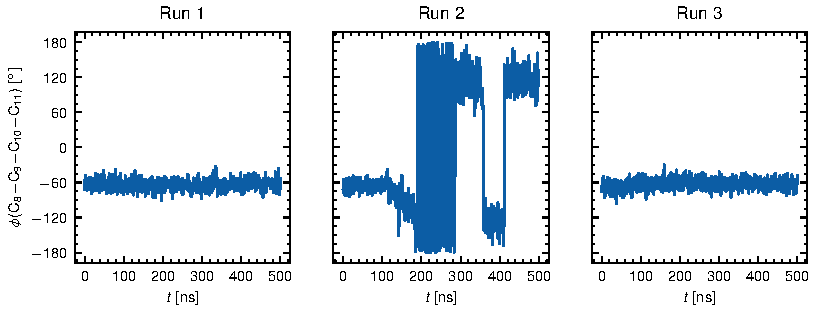
\includegraphics[width=\textwidth]{Figures/xtb_C9-C10_all.pdf}
    \end{subfigure}
    \par\bigskip
    \begin{subfigure}{\textwidth}
        \centering
        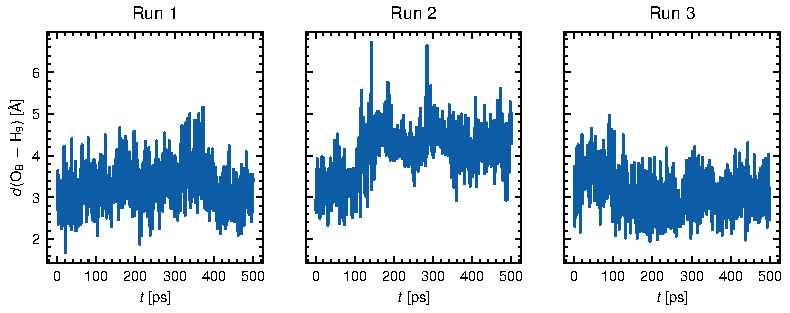
\includegraphics[width=\textwidth]{Figures/xtb_Ob-H9_all.pdf}
    \end{subfigure}
    \par\bigskip
    \begin{subfigure}{\textwidth}
        \centering
        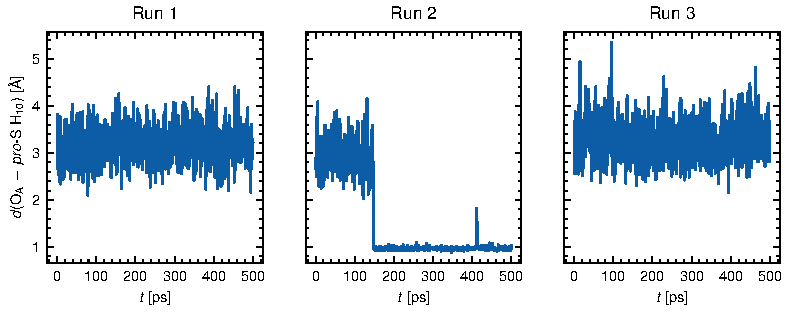
\includegraphics[width=\textwidth]{Figures/xtb_Oa-proSH10_all.pdf}
    \end{subfigure}
    \caption{Data from the three 500 ps QM/MM MD production runs of intermediate B with GFN2-xTB: value of the C$_8-$C$_9-$C$_{10}-$C$_{11}$ dihedral angle of the substrate (top); distance between the oxo oxygen (O$_{\text{B}}$) and \textit{pro}-R hydrogen on C$_9$ (H$_{9}$) that needs to get abstracted (middle); distance between the hydroxide oxygen (O$_{\text{A}}$) and \textit{pro}-S hydrogen on C$_{10}$ (bottom). Note: due to the cyclical nature of the dihedral angles the values around 180$^{\circ}$ and $-$180$^{\circ}$ correspond to the same \textit{anti} conformation.}
    \label{fig:xtb_appendix}
\end{figure}

\begin{figure}[htbp]
    \centering
    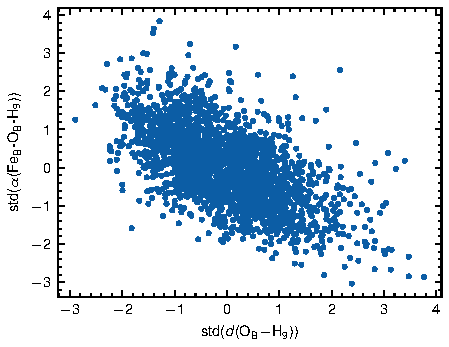
\includegraphics[width=0.6\textwidth]{Figures/2D_plot_starting_frame.pdf}
    \caption{Plot of the standardized values of the Fe$_{\text{B}}-$O$_{\text{B}}-$H$_{\text{9}}$ angle and O$_{\text{B}}-$H$_{\text{9}}$ distance during the first and third QM/MM MD production runs with GFN2-xTB of intermediate B.}
    \label{fig:starting_frame}
\end{figure}

\begin{figure}[htbp]
    \centering
    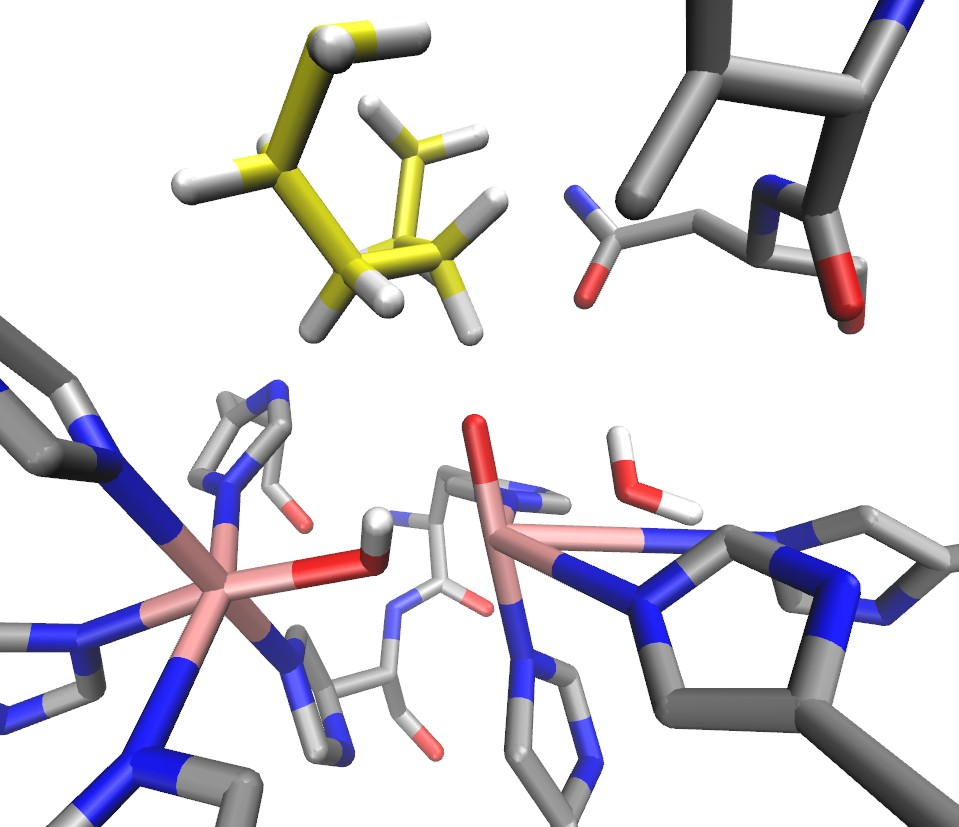
\includegraphics[width=0.7\textwidth]{Figures/pmf_window_28.png}
    \caption{Structure of the system sampled in the $\xi=0.225$ Å umbrella sampling window of intermediate B. Residues are shown as sticks. Distances are shown in Å. Colours: silver, protein carbons; red, oxygen; blue, nitrogen; white, hydrogen; yellow, carbons of stearoyl-CoA; pink, iron. Protein hydrogen atoms are left out for clarity.}
    \label{fig:pmf_window_28}
\end{figure}